\documentclass[aspectratio=169]{beamer}
\usepackage{graphicx}
\usepackage{amsmath}
\usepackage{amsfonts}
\usepackage{amssymb}
\usepackage{bm}
\usepackage{tikz}
\usepackage{hyperref}
\usepackage{multicol}

% Basic beamer setup for a clean look
\usetheme{default}
\setbeamertemplate{navigation symbols}{} % Turn off navigation symbols
\setbeamertemplate{footline}[frame number]

% Define block colors for clarity
\setbeamercolor{block title}{bg=blue!20,fg=black}
\setbeamercolor{block body}{bg=blue!5,fg=black}

% A simple command for highlighting key terms
\newcommand{\keyterm}[1]{\textbf{\textcolor{blue!70!black}{#1}}}

\title{A Statistician's Guide to the Galaxy (Fitting Zoo)}
\subtitle{An Introduction to the Statistical Foundations of SED Fitting}
\author{Future SED Fitting Workshop}
\date{\today}

\begin{document}

% --- SLIDE 0: Title Slide ---
\begin{frame}
    \titlepage
\end{frame}

% --- SLIDE 1: SED Fitting Setup (2 minutes) ---
\begin{frame}
    \frametitle{The Goal: From Photons to Physics}
    \framesubtitle{Why SED fitting is a statistical inference problem}
    \begin{columns}[T]
        \column{0.5\textwidth}
        \begin{block}{The Data}
            We observe a galaxy's light (photometry or spectra) across different wavelengths. This is our dataset, $D$.
        \end{block}
        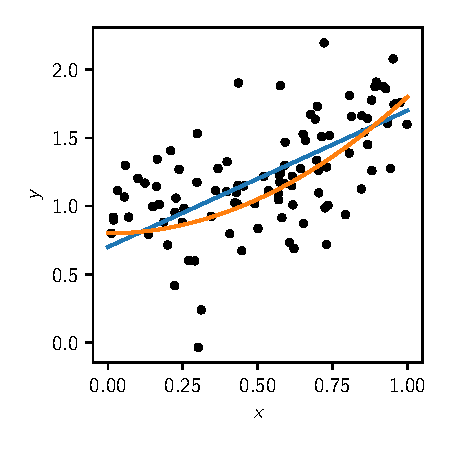
\includegraphics[width=\textwidth]{figures/data_points.pdf} % Figure from: aachen_2018/figures/data_points.pdf
        
        \column{0.5\textwidth}
        \begin{block}{The Model}
            We want to infer the underlying physical properties, our parameters, $\theta$:
            \begin{itemize}
                \item Stellar Mass ($M_*$)
                \item Star Formation History (SFH)
                \item Dust content ($A_V$)
                \item Metallicity ($Z$)
                \item ... and many more
            \end{itemize}
        \end{block}
        \begin{block}{The Challenge}
            The parameter space is often:
            \begin{itemize}
                \item \keyterm{High-dimensional}: Many parameters to fit.
                \item \keyterm{Degenerate}: Different combinations of parameters can produce similar SEDs (e.g., an old, dust-free galaxy can look like a young, dusty one).
            \end{itemize}
        \end{block}
        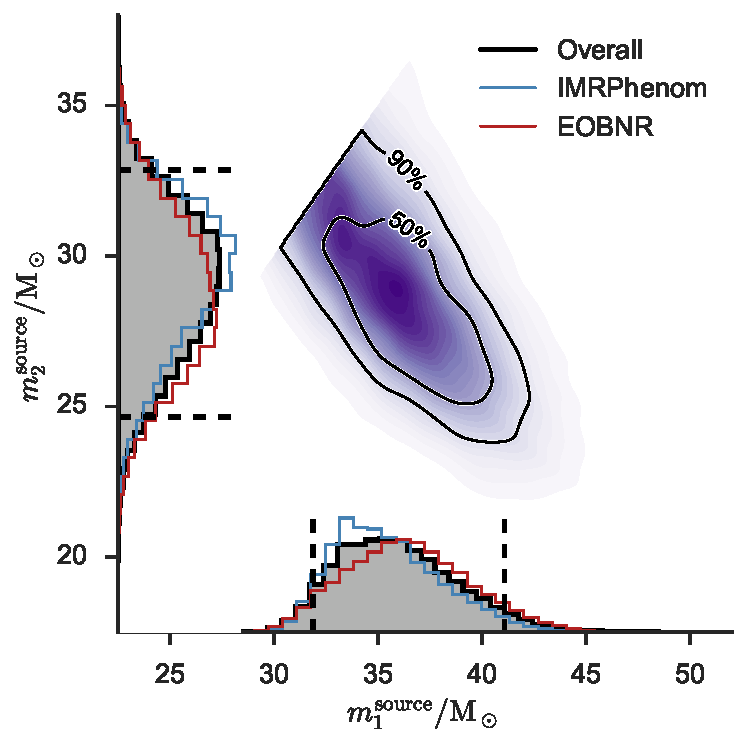
\includegraphics[width=0.8\textwidth]{figures/ligo_m1_m2.pdf} % Figure from: ift_2017/figures/ligo_m1_m2.pdf (used as an example of degeneracy)
    \end{columns}
    \vspace{1em}
    \begin{alertblock}{Key Message}
        SED fitting is not just about finding the "best" parameters; it's about mapping the entire landscape of possibilities.
    \end{alertblock}
\end{frame}

% --- SLIDE 2: Statistical Framework (2 minutes) ---
\begin{frame}
    \frametitle{The Language of Inference: Bayes' Theorem}
    \framesubtitle{How we quantify what we learn from data}
    
    \begin{center}
    \Large
    $\underbrace{P(\theta|D)}_{\text{Posterior}} = \frac{\overbrace{P(D|\theta)}^{\text{Likelihood}} \times \overbrace{P(\theta)}^{\text{Prior}}}{\underbrace{P(D)}_{\text{Evidence}}}$
    \end{center}
    \vspace{1em}
    
    \begin{columns}[T]
        \column{0.33\textwidth}
        \begin{block}{Prior}
            $P(\theta)$ \\
            What we believe about the parameters \textit{before} we see the data. Our physical assumptions.
        \end{block}
        
        \column{0.33\textwidth}
        \begin{block}{Likelihood}
            $P(D|\theta)$ \\
            The probability of observing our data, given a specific set of model parameters. This is where the physics model (e.g., from \texttt{Prospector}) connects to the data.
        \end{block}
        
        \column{0.33\textwidth}
        \begin{block}{Posterior}
            $P(\theta|D)$ \\
            What we know about the parameters \textit{after} seeing the data. It's our updated state of knowledge.
        \end{block}
    \end{columns}
    
    \vspace{1em}
    \begin{alertblock}{Key Message}
        Our goal is to find the \keyterm{posterior probability distribution}. This gives us not just best-fit values, but also the crucial uncertainties (\textit{error bars}) on our inferred parameters.
    \end{alertblock}
\end{frame}

% --- SLIDE 3: Chi-squared Maximization (3 minutes) ---
\begin{frame}
    \frametitle{The Simplest Approach: Optimization (e.g., $\chi^2$ Minimization)}
    \framesubtitle{Finding the single "best" answer}
    
    \begin{columns}[T]
        \column{0.5\textwidth}
        \begin{block}{How it Works: Hill Climbing}
            Imagine the parameter space is a landscape where lower $\chi^2$ (or higher likelihood) is "downhill".
            \begin{itemize}
                \item Start somewhere.
                \item Follow the steepest gradient downhill.
                \item Stop when you reach the bottom of a valley.
            \end{itemize}
        \end{block}
        
        \begin{block}{Advantages}
            \begin{itemize}
                \item \keyterm{Fast} and computationally cheap.
                \item Good for a quick first look.
            \end{itemize}
        \end{block}
        
        \begin{block}{Limitations}
            \begin{itemize}
                \item Only gives a single \keyterm{point estimate} (the "best fit").
                \item \textbf{No uncertainty quantification!} Where are the error bars?
                \item Can easily get stuck in a \keyterm{local minimum}, missing the true global best fit.
            \end{itemize}
        \end{block}
        
        \column{0.5\textwidth}
        \begin{center}
            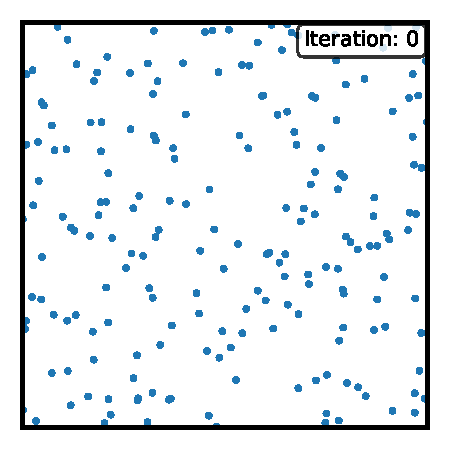
\includegraphics[width=\textwidth,page=1]{figures/himmelblau_ns.pdf} % Figure from: ini_2025/figures/himmelblau_ns (page 1)
            An optimizer might find one of these minima, but which one? And how deep/wide are they?
        \end{center}
    \end{columns}
    
    \vspace{1em}
    \begin{alertblock}{Key Message}
        Optimization is fast but gives an incomplete and potentially misleading picture. Science needs error bars.
    \end{alertblock}
\end{frame}

% --- SLIDE 4: Sampling vs Optimization (3 minutes) ---
\begin{frame}
    \frametitle{Why We Sample: Exploring the Whole Landscape}
    \framesubtitle{Getting the full story, not just the headline}
    
    \begin{columns}[T]
        \column{0.5\textwidth}
        \begin{block}{Optimization gives you the Peak}
            \begin{center}
                \includegraphics[width=0.7\textwidth,page=4]{figures/himmelblau_ns.pdf} % Figure from: ini_2025/figures/himmelblau_ns (page 4)
                \small The single best point.
            \end{center}
        \end{block}
        
        \column{0.5\textwidth}
        \begin{block}{Sampling gives you the whole Mountain Range}
            \begin{center}
                \includegraphics[width=0.7\textwidth,page=9]{figures/himmelblau_mcmc.pdf} % Figure from: ini_2025/figures/himmelblau_mcmc (page 9)
                \small A collection of points that map the entire posterior.
            \end{center}
        \end{block}
    \end{columns}
    
    \begin{block}{Why is this critical for SED fitting?}
        \begin{itemize}
            \item \keyterm{Uncertainties}: The spread of the samples tells you the uncertainty on each parameter.
            \item \keyterm{Degeneracies}: The shape of the sample cloud reveals correlations (e.g., the age-dust degeneracy).
            \item \keyterm{Multimodality}: Sampling can find all the "good" solutions, not just one.
            \item \keyterm{Model Comparison}: Some methods give us the Bayesian Evidence, allowing us to ask "Is model A better than model B?".
        \end{itemize}
    \end{block}
    
    \begin{alertblock}{Key Message}
        We sample because our physical questions require more than a single best-fit value. We need to characterize the full posterior distribution.
    \end{alertblock}
\end{frame}

% --- SLIDE 5: MCMC Sampling (4 minutes) ---
\begin{frame}
    \frametitle{The Classic Workhorse: Markov Chain Monte Carlo (MCMC)}
    \framesubtitle{The "random walker"}
    
    \begin{columns}[T]
        \column{0.5\textwidth}
        \begin{block}{How it Works (Metropolis-Hastings)}
            Imagine a "walker" exploring the parameter landscape.
            \begin{enumerate}
                \item Take a random step to a new position.
                \item If the new spot is "higher" (better likelihood), move there.
                \item If it's "lower", maybe move there anyway (with a probability that depends on how much lower it is).
                \item Repeat millions of times. The path the walker takes traces the posterior distribution.
            \end{enumerate}
        \end{block}
        
        \begin{block}{Advantages \& Limitations}
            \begin{itemize}
                \item Explores the full posterior and gives uncertainties.
                \item \textcolor{red}{Limitation:} The walker can be inefficient. It can get "stuck" in a local high-likelihood region and fail to find other, separate modes.
                \item \textcolor{red}{Limitation:} Can be slow to explore highly correlated ("banana-shaped") posteriors.
            \end{itemize}
        \end{block}
        
        \column{0.5\textwidth}
        \begin{center}
            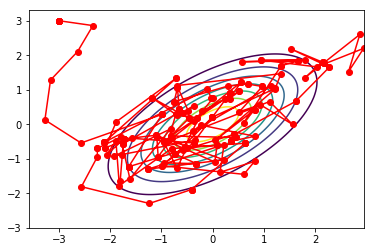
\includegraphics[width=0.8\textwidth]{figures/metropolis-hastings.png} % Figure from: ini_2025/figures/metropolis-hastings.png
            \small A single walker exploring a multimodal posterior. It finds one mode but struggles to jump to the others.
        \end{center}
    \end{columns}
    
    \begin{alertblock}{Key Message}
        MCMC is a foundational sampling method, but its simple "random walk" can be inefficient in the complex parameter spaces of SED fitting.
    \end{alertblock}
\end{frame}

% --- SLIDE 6: Ensemble Sampling (emcee) (4 minutes) ---
\begin{frame}
    \frametitle{A Better Way: Ensemble Sampling (e.g., \texttt{emcee})}
    \framesubtitle{Many walkers are better than one}
    
    \begin{columns}[T]
        \column{0.5\textwidth}
        \begin{block}{How it Works}
            Instead of one walker, we use an \keyterm{ensemble} of hundreds of walkers.
            \begin{itemize}
                \item The walkers don't move completely randomly.
                \item They propose new steps based on the positions of \textit{other} walkers in the ensemble.
                \item This allows the whole group to learn about the shape of the posterior (e.g., its correlations) and explore it more efficiently.
            \end{itemize}
        \end{block}
        
        \begin{block}{Advantages}
            \begin{itemize}
                \item Much better at exploring correlated, "banana-shaped" parameter spaces.
                \item More efficient "mixing" than a single MCMC chain.
                \item Easy to parallelize (each walker can be on a different CPU core).
            \end{itemize}
        \end{block}
        
        \begin{block}{Limitation}
            \begin{itemize}
                \item While better, the whole ensemble can still get trapped in one mode if other modes are very far away.
            \end{itemize}
        \end{block}
        
        \column{0.5\textwidth}
        \begin{center}
            
\includegraphics[width=0.8\textwidth]{figures/emcee.png} % Figure from: ini_2025/figures/emcee.png
            \small Walkers communicate to efficiently map out a correlated posterior.
        \end{center}
    \end{columns}
    
    \begin{alertblock}{Key Message}
        Ensemble samplers like \texttt{emcee} are a major improvement for many problems, especially those with parameter degeneracies.
    \end{alertblock}
\end{frame}

% --- SLIDE 7: Nested Sampling (5 minutes) ---
\begin{frame}
    \frametitle{The State of the Art: Nested Sampling (e.g., \texttt{dynesty})}
    \framesubtitle{For multimodality and model comparison}
    
    \begin{columns}[T]
        \column{0.5\textwidth}
        \begin{block}{A Radically Different Approach}
            Instead of random walking, nested sampling attacks the problem from the outside-in.
            \begin{enumerate}
                \item Start with a set of "live points" scattered across the entire \keyterm{prior}.
                \item At each step: find the point with the \textit{worst} likelihood and discard it.
                \item Replace it with a new point drawn from the prior, but with one constraint: its likelihood must be \textit{better} than the point you just discarded.
                \item This forces the set of live points to continuously "shrink" into regions of higher and higher likelihood.
            \end{enumerate}
        \end{block}
        
        \begin{block}{Key Advantages}
            \begin{itemize}
                \item Naturally handles \keyterm{multimodality}. The shrinking cloud of points will find and explore all modes simultaneously.
                \item It calculates the \keyterm{Bayesian Evidence} ($\mathcal{Z}$) as a primary output. This is essential for model comparison!
            \end{itemize}
        \end{block}
        
        \column{0.5\textwidth}
        \begin{center}
            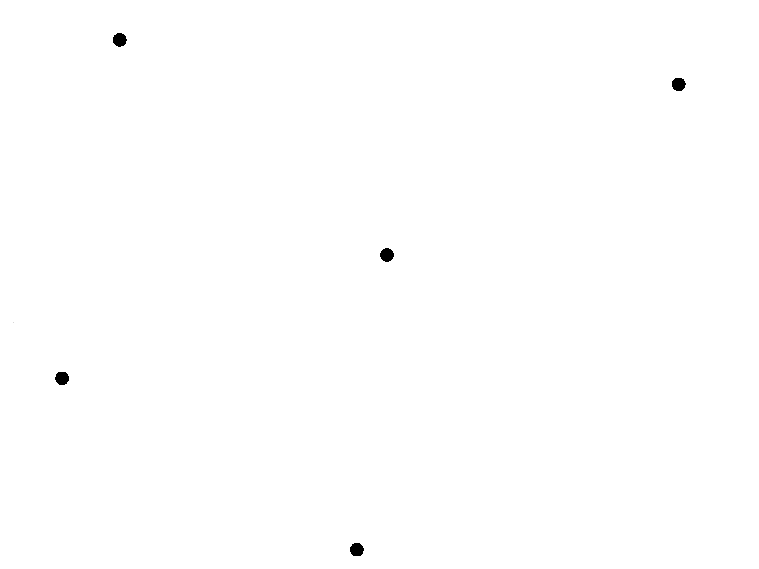
\includegraphics[width=0.8\textwidth]{figures/nested_sampling.pdf} % Figure from: aachen_2017/figures/nested_sampling.pdf
            \small The cloud of live points shrinks from the prior towards the peaks of the likelihood, mapping everything along the way.
        \end{center}
    \end{columns}
    
    \begin{alertblock}{Key Message}
        Nested sampling is powerful. It excels at exploring complex, multimodal posteriors and is the go-to method when you need to perform Bayesian model comparison.
    \end{alertblock}
\end{frame}

% --- SLIDE 8: Method Comparison (2 minutes) ---
\begin{frame}
    \frametitle{Choosing Your Tool: A Summary}
    \framesubtitle{No single best method, only the right tool for the job}
    
    \begin{center}
        \begin{tabular}{|l|c|c|c|c|}
            \hline
            \textbf{Method} & \textbf{Speed} & \textbf{Uncertainties?} & \textbf{Handles Multimodality?} & \textbf{Evidence?} \\
            \hline
            \textbf{Optimization} ($\chi^2$) & \textcolor{green!50!black}{Very Fast} & \textcolor{red}{No} & \textcolor{red}{No} & \textcolor{red}{No} \\
            \hline
            \textbf{MCMC} & \textcolor{orange}{Medium} & \textcolor{green!50!black}{Yes} & \textcolor{orange}{Poorly} & \textcolor{red}{No} \\
            \hline
            \textbf{Ensemble} (\texttt{emcee}) & \textcolor{orange}{Medium} & \textcolor{green!50!black}{Yes} & \textcolor{orange}{Okay} & \textcolor{red}{No} \\
            \hline
            \textbf{Nested} (\texttt{dynesty}) & \textcolor{red}{Slower} & \textcolor{green!50!black}{Yes} & \textcolor{green!50!black}{Excellently} & \textcolor{green!50!black}{Yes!} \\
            \hline
        \end{tabular}
    \end{center}
    
    \vspace{2em}
    
    \begin{block}{Practical Guidance}
        \begin{itemize}
            \item \textbf{Quick exploration / Sanity check?} $\rightarrow$ Use Optimization.
            \item \textbf{Simple, well-behaved posterior?} $\rightarrow$ \texttt{emcee} is a great choice.
            \item \textbf{Complex, possibly multimodal posterior?} $\rightarrow$ Use \texttt{dynesty}.
            \item \textbf{Need to compare different physical models?} $\rightarrow$ You \textit{must} use Nested Sampling to get the evidence.
        \end{itemize}
    \end{block}
    
    \begin{alertblock}{Key Message}
        Your choice of statistical method depends on your scientific question and the expected complexity of your model.
    \end{alertblock}
\end{frame}

% --- SLIDE 9: AI in Scientific Code Development (2 minutes) ---
\begin{frame}
    \frametitle{The Future: AI in Scientific Code Development}
    \framesubtitle{How these tools themselves are evolving}
    \begin{columns}[T]
        \column{0.5\textwidth}
        \begin{block}{The Real AI Revolution: LLMs as Translators}
            The biggest impact of AI may not be in analyzing data, but in helping us write the code to do it.
            \begin{itemize}
                \item \keyterm{Automated code translation}: LLMs can help port legacy Fortran/C++ models to modern, GPU-friendly frameworks like JAX or PyTorch.
                \item \keyterm{Automatic Differentiation}: These modern frameworks give us model gradients "for free," enabling more powerful sampling methods (like Hamiltonian Monte Carlo).
                \item \keyterm{Neural Emulators}: If your model is very slow to run, you can train a neural network to emulate it, providing a massive speed-up for sampling.
            \end{itemize}
        \end{block}
        
        \column{0.5\textwidth}
        \begin{block}{The 80/20 Rule of Scientific Work}
            \begin{itemize}
                \item \textbf{80\% "boring" tasks}: Writing code, debugging, drafting papers, managing data...
                \item \textbf{20\% "hard thinking"}: The actual scientific insight.
            \end{itemize}
            AI's biggest immediate impact is automating and accelerating the 80\%, freeing up human time for the 20\%.
        \end{block}
        
        \begin{block}{Challenges}
            As we rely more on AI-generated code, we must be vigilant.
            \begin{itemize}
                \item Ensuring correctness and reproducibility.
                \item Maintaining interpretability of our models and methods.
            \end{itemize}
        \end{block}
    \end{columns}
    
    \begin{alertblock}{Key Message}
        AI is not just a tool for analysis; it's fundamentally changing how we develop, optimize, and deploy our scientific software.
    \end{alertblock}
\end{frame}

% --- SLIDE 10: Conclusions (1 minute) ---
\begin{frame}
    \frametitle{Conclusions \& What's Next}
    
    \begin{block}{Key Takeaways}
        \begin{itemize}
            \item SED fitting is a problem of \keyterm{statistical inference}, not just optimization.
            \item The goal is the full \keyterm{posterior distribution}, which gives us parameters \textit{and} their uncertainties.
            \item \keyterm{Sampling} methods are the tools we use to map out the posterior.
            \item The choice of sampler—from MCMC to Ensemble to Nested—depends on the complexity of your problem and whether you need to do \keyterm{model comparison}.
        \end{itemize}
    \end{block}
    
    \vspace{2em}
    
    \begin{center}
        \huge Thank you!
    \end{center}
    
    \vspace{1em}
    
    \begin{alertblock}{Next Up: David Yallup on "GPU Accelerated Nested Sampling"}
        Now that we know \textit{why} nested sampling is so powerful, we'll hear about how to make it \textit{fast}!
    \end{alertblock}
\end{frame}

\end{document}